\section{Motivation}
Albeit the goal stated in the introduction chapter is focused at the method of obtaining quality agents, the motivation for such endeavor must be kept in mind. It would be beneficiary for a number of use cases to obtain a system which, when provided with a sufficient description of an environment and capabilities of agents, could be used to produce ready to be implemented Behavior Trees capable of performing given assignments. Arguably, additional overhead due to implementing the environment \& agents specifications and task description must be taken into account when considering using such system, potentially making the method unfeasible in scenarios when the time is of essence. Even then however, one has to weight initial investment into such project against manually designing and adjusting the AI.

Additionally, there is also one critical advantage to using evolutionary learning methods: the possibility of early termination through end condition. With the right fitness function the option to take an undeveloped tree as a template and improve it becomes perfectly possible. This can be useful in more sophisticated problems, when manual tuning will complement evolutionary method's solution. % to be perfectly honest, I'm not sure if this is the appropriate place to be making such claims - I mean discussing practical advantages.
\section{Formulating a Task}
In order to properly assess feasibility of the system in making, a common task had to be constructed to compare different variations of a system in-making against each other. Scenario type chosen for this task was a resource gathering, a domain referred in \cite{cooperationstateoftheart} as \textbf{foraging}.

The premise of this particular scenario was as follows: a certain amount of numbered resource markers (portrayed as flags in the simulation) were scattered across the simulated environment resembling a warehouse. The agents, starting from designated spawn points, are tasked with claiming as many of them as possible against a fixed time limit. \textit{Claiming} in this case was a process consisting of approaching a certain vicinity of a marker, at which point it was despawned and marked off as \textit{captured} by an agent initiating the claiming. Making the process instantaneous ensured that markers would be claimed on FCFS (\textit{First-Come, First-Served}) basis. Accompanying the evolutionary agent was the human-defined tree, filling a role of a rival - in a competitive scenario - or a partner - in the cooperative one.

While the particulars were a subject to fine-tuning numerous times, Figure \ref{fig:x taskoverview} presents the initial schema of agents' and markers' spawn points.
\begin{figure}[h]
    \centering
    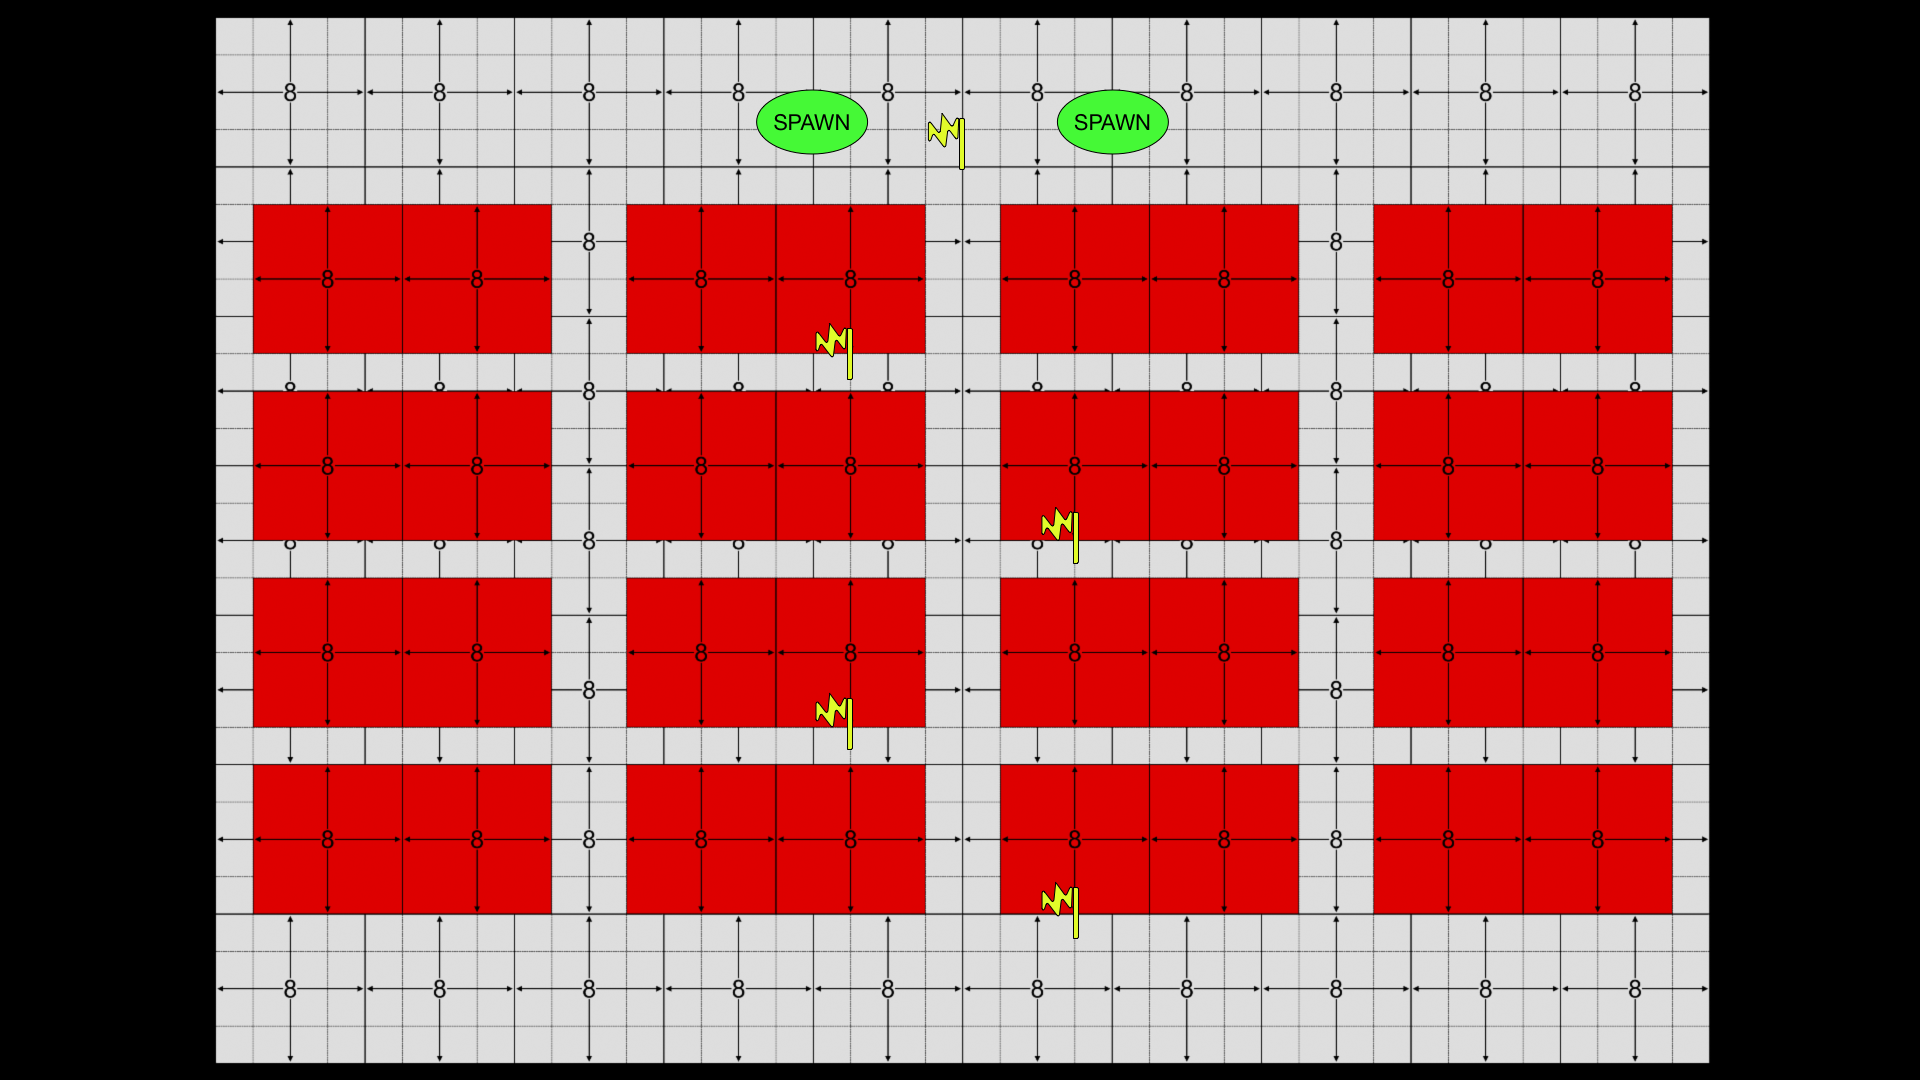
\includegraphics[scale=0.2]{taskoverview}
    \caption{Initial positioning of agents' starting points and resource markers.}
    \label{fig:x taskoverview}
\end{figure}
\section{Incorporating Genetic Programming}
The Genetic Programming module was built on top of FRAIL's existing features, substantially changing the usual flow of execution to make it suitable for learning processes. Initialization, evaluation and reproduction steps are all done internally, with evaluation being a step when the actual simulations are run. Since the population was being tested sequentially and the maximum time one could run was 20s (with the possibility to end early, in case all markers were gathered before that time), some testing would take more than 48 hours to complete. We decided to increase update frequency of the simulations tenfold, thus guaranteeing simulations would complete after maximum of 2s.
\subsection{Representation}
In the interest of avoiding integrity requirements and semantic incoherences (which would be undoubtedly caused by genetic operators), specimen are instances of a specialized class, separated from the actual Behavior Tree class responsible for tree execution. These trees are then parsed during evaluation step to a ``regular'' Behavior Tree that is injected to an AI Controller in the simulation.

This simplified implementation allowed for easier manipulation of the trees' components. The nodes are distinguished by their type, but otherwise have all parameters required to operate. While this poses a serious data redundancy, the possibility of freely adding additional node types and ease of operations made this option highly desirable.
\subsection{Genetic Operations}
% add comment?
\subsubsection{Initialization}
The population starts as a set of randomly generated specimen of varying size and depth. Each tree generation starts with a random Composite node in root, then the decision is made a at each further step to either add a random Action / Condition node to current root's children or recursively create a random subtree, all bound by a maximum size and maximum depth allowed. This approach provides a varied population while maintaining good balance of Action / Condition and Composite nodes.
\subsubsection{Selection}
The selection method of choice is a regular implementation of Tournament Selection. At each step, a random sample of a given size is selected from the current population and sorted according to a fitness value of the specimen. The first individual from this set is selected for Reproduction purposes.
\subsubsection{Crossover}
On each iteration, two selected specimen have a chance (determined by crossover rate parameter) to produce two children which will be put into the next generation instead of them. The crossover itself is a single-point version, implemented as a exchange of randomly selected nodes (one from each tree) without minding their type nor location.
\subsubsection{Mutation}
Genetic Programming framework offers two methods of mutation: micro- and macromutation, previously explained in chapter \ref{chapter_background}. Both were implemented: initially, only the possibility for the tree to undergo micromutation is tested - that is implemented by resetting randomly chosen node's parameters to a random values. However, each tree selected for a micromutation process (probability of which is dictated by a mutation rate) has a chance to undergo a macromutation process instead - that, in turn, is determined by a separate, macromutation rate. In this case, micromutation step is replaced entirely with ``Headless Chicken'' mutation.
\subsubsection{Fitness function}
Due to the format of the experiments, where solutions to two different scenarios were explored separately, used fitness function varied between experiments. There is, however, a number of factors that were considered relevant to the fitness of the specimen that can be presented now. These were:
\begin{itemize}
    \item \textbf{Number of markers gathered} - a number of resource markers gathered.
    \item \textbf{Time to completion} - how much time did it take to finish the simulation (i.e. how much time has elapsed until all the markers were claimed).
    \item \textbf{Size of a Tree} - how many nodes were in the tree.
\end{itemize}
The first characteristic ended up being relevant only in the competitive scenario, where agents were to compete in claiming the markers: the number of claimed resources was, in fact, the defining characteristic. The relevance of the two following features, however, was common to both cases: the best solution is expected to finish the task as close to the shortest time as possible, while pressuring the algorithm to keep decreasing the size of a tree was done in the interest of both readability (and, with that, ease of modification) and execution time.
\section{Behavior Tree}
The solution produced by the algorithm had to be \textit{translated} to an actual Behavior Tree representation used in the simulations for the reasons discussed earlier in this chapter. The process was, however, a part of the usual workflow and required no interaction from the user.

Specimen were built from only three kinds of nodes: \textit{Selector}, \textit{Sequence} and one Action - \textit{goToFlag(flagNumber)}. This decision was made based on relative simplicity of the task, not requiring elaborate choice in actions. \textit{goToFlag} automatically chooses the optimal route to the selected path and, when the actor approaches capturing distance, attempts to claim the marker. Note that there is no information provided on the marker still being in the chosen place, as well as no knowledge at all about the state of the board. Agents operate thus in an environment with incomplete information, with the position of the markers being the only information available.

Furthermore, \textit{goToFlag} Action provided additional two variants, tied with the identifier argument. While values of 1-7 would select one of the existing markers, values $-1$ and $0$ held special meaning: -1 would set the course on the furthest \textit{available} (non-claimed) marker, while the latter would select nearest one. This was done in order to see if that level of abstraction would be preferable in certain situations, acting with critical timing against unchanging reference agent. The listing below presents pseudocode algorithm of \textit{goToFlag} Action.

\begin{lstlisting}[language=C++]
actionGoToFlag(int identifier)
{
    if (identifier ==  -1)
        goToFurthestFlag()
    else if (identifier == 0)
        goToNearestFlag()
    else
        goToFlag(identifier - 1)
}
\end{lstlisting}
\section{Environment}
\subsection{Introduction}
\textbf{FRAIL} (Framework for AI Laboratories) is a platform developed in-house at Wroclaw's University of Technology (PWR) for purposes of testing artificial adversaries in shooter games. \cite{frailweb}

As an in-house project, users were able to freely access and change the source code, modifying existing controllers or creating new ones. Since its launch, FRAIL has seen use as a didactic aid during Artificial Intelligence classes and bootstrap for various AI-related projects, including evaluation by a video game development and publishing company, Techland for internal use. % citation needed?

In order to fully utilize the platform's capabilities, substantial changes have been made to FRAIL's engine in one of the previous projects, allowing for the entire process of Genetic Programming to be executed on the platform itself. A Behavior Tree implementation and representation related modules were taken from current version of FRAIL and the project was reverted to one of the earlier versions to reduce bloating. Genetic Programming module was implemented as a ``building block'' that could be placed on any map operating in ``Capture the Flag'' mode. Exploiting FRAIL's scripting behaviors and usage of RTTI (Run-Time Type Identification), a number of convenience changes were introduced to control the environment and algorithm parameters.
\subsection{Map overview}
The task planned for the agents can be described as a resource retrieval. To simulate this scenario, a map resembling a warehouse has been planned and prepared for use. Figure \ref{fig:x simmaprender} presents a 3D render of a finished map, while a top-down view, featured on Figure \ref{fig:x simmaptopdown} will be referred to further describe the design.

\begin{figure}[h]
    \centering
    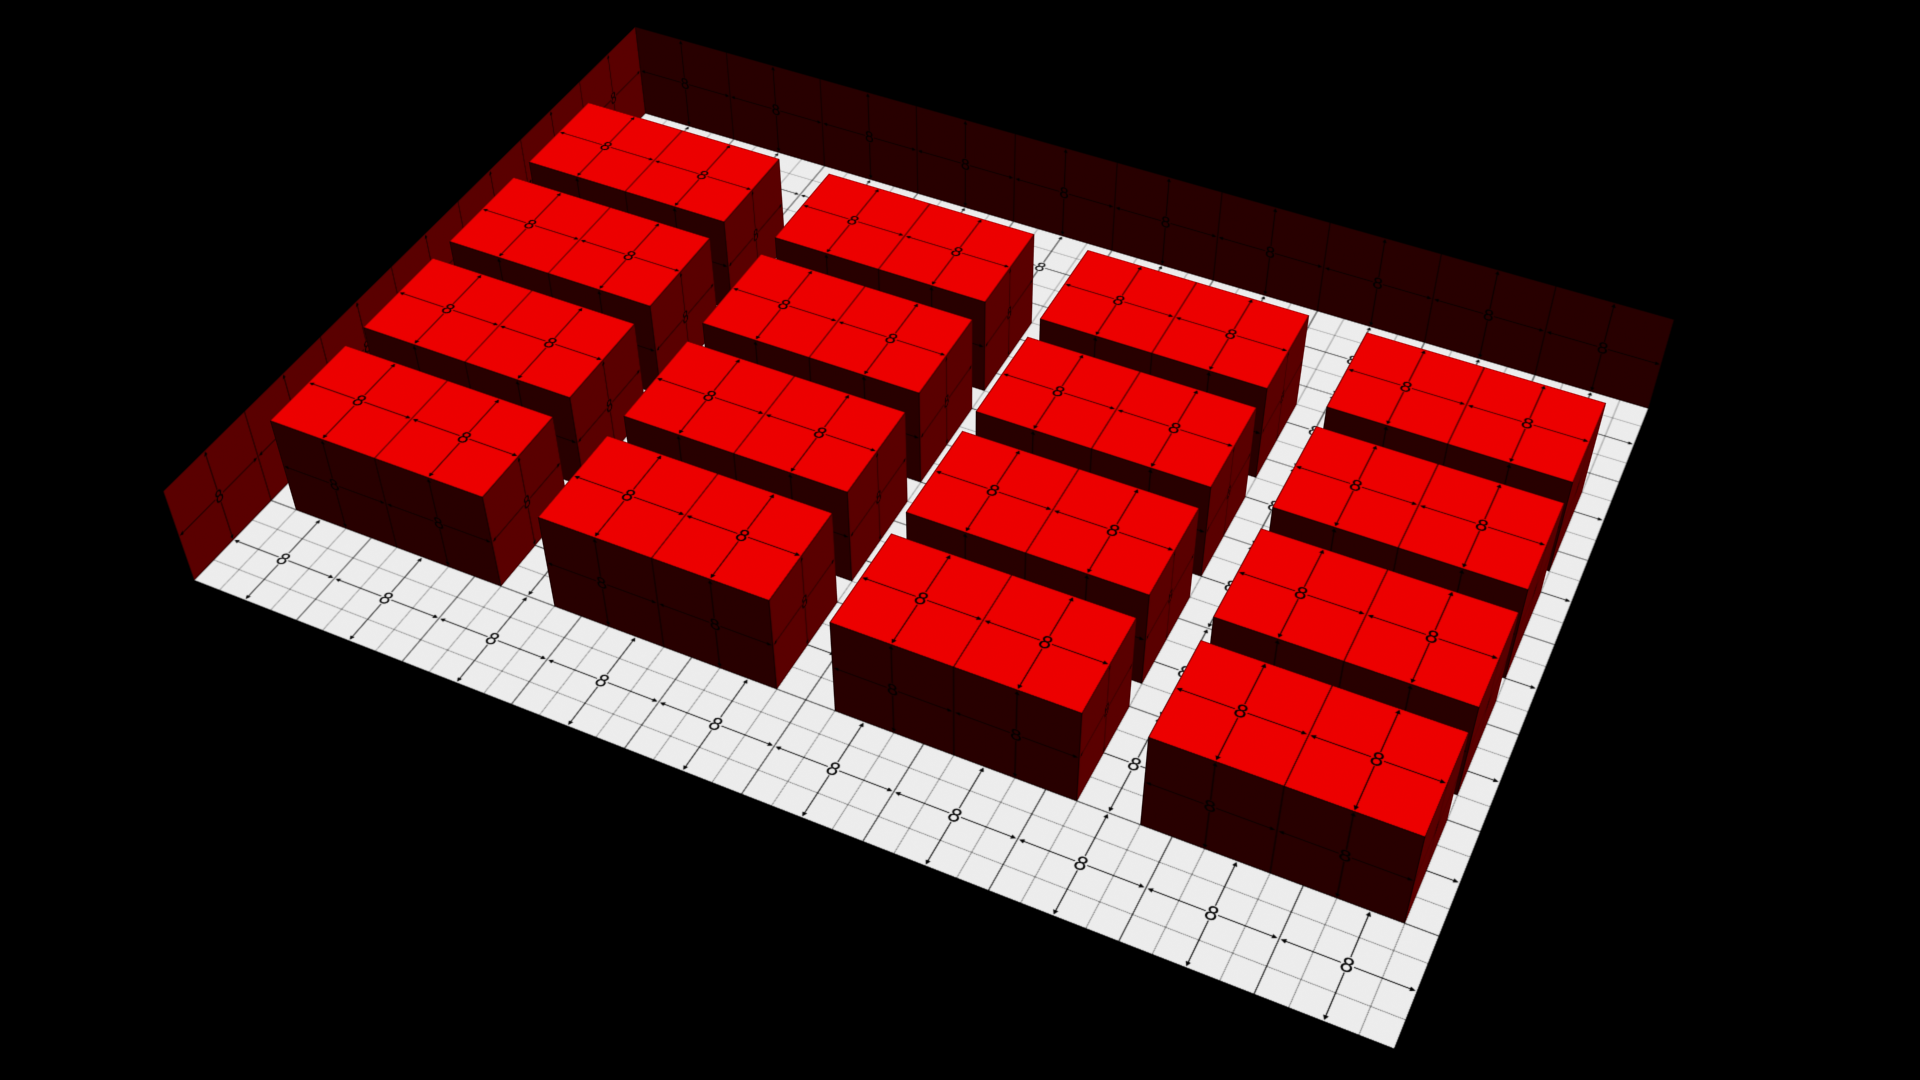
\includegraphics[scale=0.2]{frailmaprender}
    \caption{A rendering of scenery}
    \label{fig:x simmaprender}
\end{figure}

\begin{figure}[h]
    \centering
    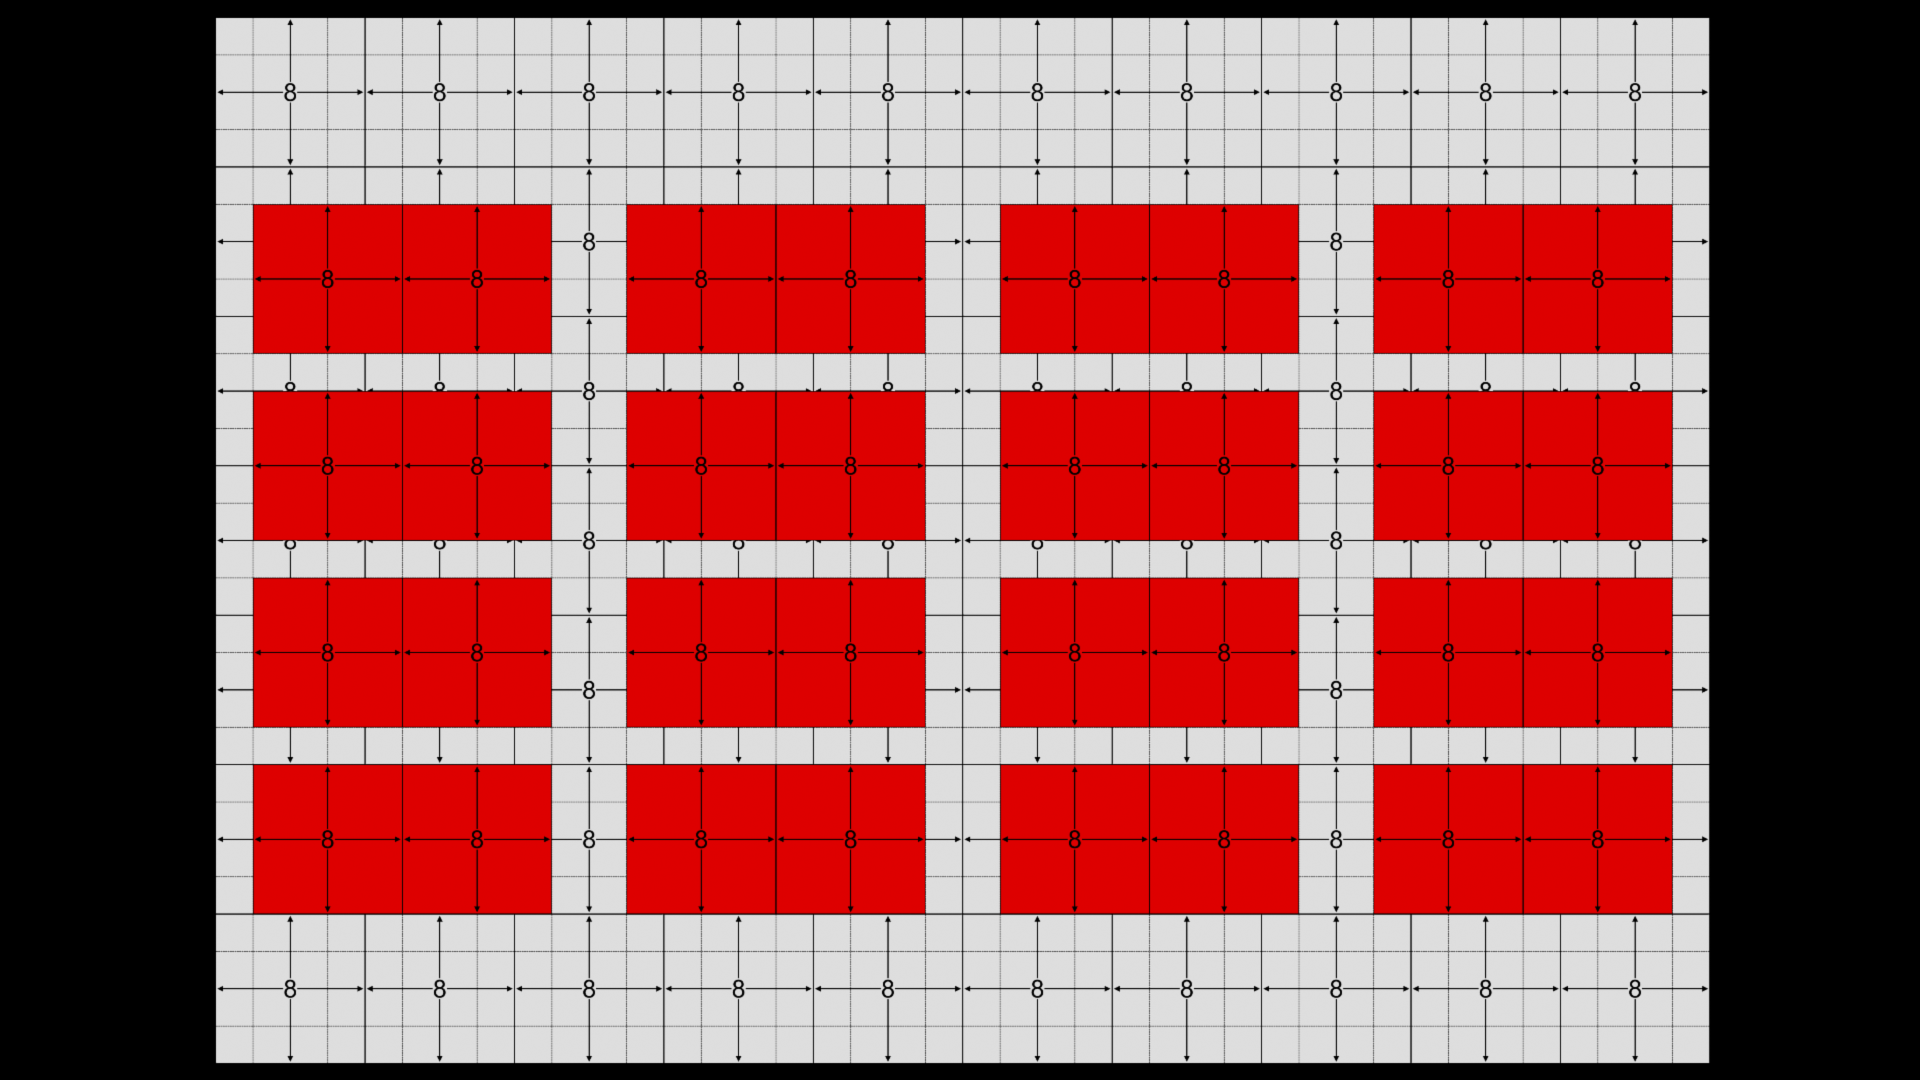
\includegraphics[scale=0.2]{frailmaptopdown}
    \caption{A top-down view of the map}
    \label{fig:x simmaptopdown}
\end{figure}

The map was designed with two to four agents in mind, with the possibility of scaling up when needed. Its shape is rectangular, measuring 80 on 56 simulation units. Over the middle section, 14 cuboid structures were placed symmetrically to act as storage containers / shelve-holding space, with access points along every edge. This placement allowed to make use of narrow alleys between containers in order to create potential conflict points, and positioning resources right next to them would hopefully allow for more faithful representation of a real-world resource gathering problem.
% I'm not sure what exactly belongs here. For instance: I should note that introduction of GP to the platform was done beforehand, since I made only the GP part, it was my partner who integrated it within frail. There were no publications, however, since it was only a class project.
